% !TeX root = ../report.tex
% !TeX spellcheck = en-US
% !TeX encoding = UTF-8


\chapter{DESIGN VALIDATION}\label{chap:design validation}

The actual implementation of the controller framework, as set out in Section~\ref{sec:controller}, is dubbed
``ohCaptain''. The source code is provided in Appendix~\ref{app:ohcaptain source code}. The code repository can be found
at \url{https://github.com/jellespijker/ohCaptain}. This includes build scripts and device-tree overlays for an arm
embedded \gls{acr-SBC} of the \gls{acr-BBB} variant.

Validation of the controller performance is an significant benchmark. In particular the localization under uncertainty
challenge. This could either be done in a field test with the actual crawler, or in a virtual simulation environment.
Provided that the simulated environment is an accurate representation of the physical world.

\noindent This chapter describes the simulation setup in Section~\ref{sec:simulation}. The final results are discussed
in Section~\ref{sec:results}.

\begin{RoyalNote}{BACKGROUND}
    The crawler which was available at the beginning of this project, was for various unrelated reasons disassembled,
    before any actual testing could be performed. Roughly around the same time, the working environment and contract 
    of the author changed as well. This forced validation to be performed in a simulation.
\end{RoyalNote}


\section{SIMULATION}\label{sec:simulation}

In order to tell something meaningful about the performance of a controller, it has to be subject to the same physical
processes as it would in real-life, albeit in virtual form. Section~\ref{sec:motion model} lists all known external
forces which are interacting with the crawler, and concludes that the dynamic properties of the drive-train and soil
play a huge part in the kinematic behavior of the crawler. There are a couple of physics simulation engines that which
are candidates for usage in this project:  \href{http://gazebosim.org/}{Gazebo},
\href{https://projectchrono.org/}{Project Chrono}, \href{https://pybullet.org/wordpress/}{Bullet} and
\href{https://developer.nvidia.com/gameworks-physx-overview}{PhysX}.

From this list, only \gls{gls-Project_Chrono} has an existing framework which takes into account soil dynamic
behavior and
terramechanics. This is either simulated using \gls{acr-DEM} or granular approach. Where each particle of sand is
an individual body and is represented as a spherical rigid bodies whose orientation is captured by Euler parameters.
For each time step a complete geometric characterisation of all contacting particles is then obtained using collision
detection and inter-particle normal contact forces are calculated by allowing small inter-penetrations using a penalty
method for \gls{acr-DEM}. Were the normal contact force is based on Hertz law and friction forces are calculated using
the Coulomb limit~\cite{recuero_high-fidelity_2017}\cite{serban_co-simulation_2018}. This method is computational heavy
and more suitable for detailed modelling.

An alternative method is the \gls{acr-SCM}, based upon the familiar Becker-Wong model. The model provides a
semi-empirical approach to the simulation of soft soil. It offers high speed of simulation and it's accurate enough for
many scenarios. It has the following attributes: it depends on parameters (the same that are used in the Bekker- Wong
model); it can generate 3D ruts on terrains of variable height; it takes into account multi-pass hardening when wheels
generate intersecting ruts; it can work with irregular triangle-based terrain meshes; it supports an optional refinement
of the terrain mesh to capture fine details like tire threads and lugs and it's compatible with deformable tires and
generic shapes like obstacles, track shoes of tanks, etc. On the downside, the new soil model cannot simulate lateral
bulldozing effects like those happening when a tracked vehicle steers in-place and pushes material apart~
\cite{tasora_overview_2018}. This means that the proposed slip-prediction method can't be used in this simulation.

A big part of the physics engine, Project Chrono, is the autonomous vehicle support. This is set-up according to 
well-known \gls{acr-OOP} practices (such as polymorphism), using virtual overrides in classes that represent physical
bodies. A custom model for different models of a drive-train, body, wheels/tracks and controller can defined and 
connected as needed. Where the behavior of that individual model can be thought of as black box as long as the 
interface with the components it connects to, is maintained. Section~\ref{sec:simulation model} describes the 
modelling of the drive-train in detail. The support of realistic sensor characteristic are not yet implemented in 
Project Chrono since a big part of the validation is measuring the performance of a Kalman Filter. An extension for 
\gls{gls-Project_Chrono} had to be written, which allows for the modelling of sensor behavior. This extension is 
described in Section~\ref{sec:sensor simulation}.

\subsection{SENSOR SIMULATION}\label{sec:sensor simulation}

One of the biggest challenges and risks determining how it should deal with uncertainties and errors introduced by 
the inherent behavior and limits of the sensors. \gls{gls-Project_Chrono} is an established and mature physics 
simulation engine which is written in C++. It consists of multiple modules. Simulating the behavior of an autonomous 
vehicle requires usage of the Core module, where Physics, Geometric and Collision objects are defined and the Vehicle
module, containing among others objects for a Driver system, Powertrain, Terrain and Steering. The orientation and 
position for every object can be tracked, logged and plotted. These values represent continual ideal states, governed
by the simulated physical laws. Simulating a controller with these values as input signals isn't representative for 
the real world.

The code for \gls{gls-Project_Chrono} has been released under a BSD-3 clause, this allows for modification and
distribution of
code for private and commercial use. An extension for realistic sensor behavior is written for this project en released
as open-source for others to use. The extension library makes it possible to attach a virtual sensor somewhere on a
frame, define which native signals it should use. For instance: acceleration of the sensors local coordinate system
vector \gls{sym-a_z_k} compared to the global coordinate system. These values can then be transformed by routing it
through different signal transformations, which represent typical errors. The transformed values can then be used as
input for a controller and/or logged for post-processing. These typical errors are sensors characteristic which are
discussed in Section~\ref{sec:sensors}. An inventory of the different errors is listed in the below. The subsequent
sections describe which modification are used for sensors in this project.

\begin{RoyalTable}{X[2,l,m] X[4,l,m]}
    \RoyalHeader{ERROR||DESCRIPTION}
    \RoyalRow{Noise|The input signal is transformed by adding a noise signal to it. The noise can either be generated
    with a random Gaussian distribution or a uniform distribution}
    \RoyalRow{Digitize|The resolution of the incomming signal is lowered to a specified amount of bits, this will
    reduce the precision}
    \RoyalRow{Bias|A constant offset is added to signal, simulating a drift}
    \RoyalRow{Transform|A signal can be transformed with a tranformation matrix (stretching, squeezing, rotating,
    shear, reflect, etc.), simulating \gls{gls-hard-iron} effect with a skew transform matrix for instance}
    \RoyalRow{Hysteresis|A signal is delayed simulating a lag in response of the system}
\end{RoyalTable}

\subsubsection{ACCELEROMETER}

% noise /digitize
An \gls{gls-accelerometer} is subjective to the effects of temperature and discretization of an analog signal to its
digital representation\cite{abyarjoo_implementing_2015}. The noise is analog in nature and is therefor model before the
discretization.

\begin{RoyalFigure}[h, label=fig:accelerometersim]{SIGNAL TRANSFORM ACCELEROMETER}
    \resizebox{0.5\textwidth}{!}{
    \begin{tikzpicture}[auto, node distance=4cm,>=latex', align=center]
        \node[block] (digitize) {Digitize};
        \node[lbl] (bits) at ($(digitize.north)+(0, 1)$) {\tiny Bits};
        \draw[-latex] (bits) -- (digitize);

        \node[block, left of=digitize] (noise) {Noise};
        \node[lbl] (mean) at ($(noise.north)+(0.5, 1)$) {\tiny Mean};
        \draw[-latex] (mean) -- ($(noise.north)+(0.5, 0)$);
        \node[lbl] (std dev) at ($(noise.north)+(-0.5, 1)$) {\tiny Std. dev.};
        \draw[-latex] (std dev) -- ($(noise.north)+(-0.5, 0)$);

        \node[input, left of=noise, xshift=2cm] (input) {};
        \node[output, right of=digitize, xshift=-2cm] (output) {};

        \draw[-latex] (input) -- (noise) node[midway] {\gls{sym-y_k}};
        \draw[-latex] (noise) -- (digitize);
        \draw[-latex] (digitize) -- (output) node[midway] {\gls{sym-y_k_prime}};
    \end{tikzpicture}}
\end{RoyalFigure}

\subsubsection{GYROSCOPE}

The \gls{gls-gyroscope} is subject to a drift along its rotational axis or induced by the rotation of the earth. Noise
from different sources is also added to the signal. Signals from modern gyroscopes are interpreted on a microcontroller,
which convert the analog values to digital levels.

\begin{RoyalFigure}[htb, label=fig:gyroscopesim]{SIGNAL TRANSFORM GYROSCOPE}
    \resizebox{0.5\textwidth}{!}{
    \begin{tikzpicture}[auto, node distance=4cm,>=latex', align=center]
        \node[input] (input) {};

        \node[sum, right of=input] (s1) {};

        \node[block, right of=s1, xshift=-2cm] (noise) {Noise};
        \node[lbl] (mean) at ($(noise.north)+(0.5, 1)$) {\tiny Mean};
        \draw[-latex] (mean) -- ($(noise.north)+(0.5, 0)$);
        \node[lbl] (std dev) at ($(noise.north)+(-0.5, 1)$) {\tiny Std. dev.};
        \draw[-latex] (std dev) -- ($(noise.north)+(-0.5, 0)$);

        \node[block, below of=noise, yshift=2cm] (bias) {Bias};
        \node[lbl] at ($(bias.south)+(0, -0.5)$) (offset) {\tiny Offset};
        \draw[-latex] (offset) -- (bias);

        \node[sum, right of=noise] (s2) {};

        \draw[-latex] (s1) |- (bias);
        \draw[-latex] (bias) -| (s2);

        \node[block, right of=s2, xshift=-2cm] (digitize) {Digitize};
        \node[lbl] (bits) at ($(digitize.north)+(0, 1)$) {\tiny Bits};
        \draw[-latex] (bits) -- (digitize);

        \node[output, right of=digitize, xshift=-2cm] (output) {};

        \draw[] (input) -- (s1) node[midway] {\gls{sym-y_k}};
        \draw[-latex] (s1) -- (noise);
        \draw[] (noise) -- (s2);
        \draw[-latex] (s2) -- (digitize);
        \draw[-latex] (digitize) -- (output) node[midway] {\gls{sym-y_k_prime}};
    \end{tikzpicture}}
\end{RoyalFigure}

\subsubsection{MAGNETOMETER}

A \gls{gls-magnetometer} experience distortions in its fields, Either due to \gls{gls-soft-iron} or \gls{gls-hard-iron}
effects. These manifest in an elliptical nature, a skewed circle. A transformation matrix mimics those distortions. The
sensor is also sensitive to background distortions, resulting in noise in the signal. This signal is also digitized.

\begin{RoyalFigure}[htb, label=fig:magnetometersim]{SIGNAL TRANSFORM MAGNETOMETER}
    \resizebox{0.5\textwidth}{!}{
    \begin{tikzpicture}[auto, node distance=4cm,>=latex', align=center]
        \node[block] (digitize) {Digitize};
        \node[lbl] (bits) at ($(digitize.north)+(0, 1)$) {\tiny Bits};
        \draw[-latex] (bits) -- (digitize);

        \node[block, left of=digitize] (noise) {Noise};
        \node[lbl] (mean) at ($(noise.north)+(0.5, 1)$) {\tiny Mean};
        \draw[-latex] (mean) -- ($(noise.north)+(0.5, 0)$);
        \node[lbl] (std dev) at ($(noise.north)+(-0.5, 1)$) {\tiny Std. dev.};
        \draw[-latex] (std dev) -- ($(noise.north)+(-0.5, 0)$);

        \node[block, left of=noise] (transform) {Transform};
        \node[lbl] (matrix) at ($(transform.north)+(0, 1)$) {\tiny Matrix};
        \draw[-latex] (matrix) -- (transform);

        \node[input, left of=transform, xshift=2cm] (input) {};
        \node[output, right of=digitize, xshift=-2cm] (output) {};

        \draw[-latex] (input) -- (transform) node[midway] {\gls{sym-y_k}};
        \draw[-latex] (transform) -- (noise);
        \draw[-latex] (noise) -- (digitize);
        \draw[-latex] (digitize) -- (output) node[midway] {\gls{sym-y_k_prime}};
    \end{tikzpicture}}
\end{RoyalFigure}

\subsubsection{ENCODER}

An encoder measures events in time, these events are usually triggers generated by a photodiode, which is
intermittently blocked or exposed from a light source with the use of a code disk. \citet{j_borenstein_where_1996} state
these relative inexpensive devices are well-suited for velocity feedback sensors in medium-to-high control systems, but
run into noise and stability problems at slow velocities due to quantization errors.

\begin{RoyalFigure}[htb, label=fig:encodersim]{SIGNAL TRANSFORM ENCODER}
    \resizebox{0.5\textwidth}{!}{
    \begin{tikzpicture}[auto, node distance=4cm,>=latex', align=center]
        \node[block] (digitize) {Digitize};
        \node[lbl] (bits) at ($(digitize.north)+(0, 1)$) {\tiny Bits};
        \draw[-latex] (bits) -- (digitize);

        \node[block, left of=digitize] (noise) {Noise};
        \node[lbl] (mean) at ($(noise.north)+(0.5, 1)$) {\tiny Mean};
        \draw[-latex] (mean) -- ($(noise.north)+(0.5, 0)$);
        \node[lbl] (std dev) at ($(noise.north)+(-0.5, 1)$) {\tiny Std. dev.};
        \draw[-latex] (std dev) -- ($(noise.north)+(-0.5, 0)$);

        \node[input, left of=noise, xshift=2cm] (input) {};
        \node[output, right of=digitize, xshift=-2cm] (output) {};

        \draw[-latex] (input) -- (noise) node[midway] {\gls{sym-y_k}};
        \draw[-latex] (noise) -- (digitize);
        \draw[-latex] (digitize) -- (output) node[midway] {\gls{sym-y_k_prime}};
    \end{tikzpicture}}
\end{RoyalFigure}

\subsubsection{PRESSURE SENSOR}

\citet{liptak_instrument_2003} mentions that \gls{gls-pressure-sensor} are subject to hysteresis of there signal because
of the material properties of the membrane and its ability to bounce back. The electrical components of these sensors
are also subjective to background noise. The final filter digitizes the signal.

\begin{RoyalFigure}[htb, label=fig:pressuresensorsim]{SIGNAL TRANSFORM PRESSURE SENSOR}
    \resizebox{0.5\textwidth}{!}{
    \begin{tikzpicture}[auto, node distance=4cm,>=latex', align=center]
        \node[block] (digitize) {Digitize};
        \node[lbl] (bits) at ($(digitize.north)+(0, 1)$) {\tiny Bits};
        \draw[-latex] (bits) -- (digitize);

        \node[block, left of=digitize] (noise) {Noise};
        \node[lbl] (mean) at ($(noise.north)+(0.5, 1)$) {\tiny Mean};
        \draw[-latex] (mean) -- ($(noise.north)+(0.5, 0)$);
        \node[lbl] (std dev) at ($(noise.north)+(-0.5, 1)$) {\tiny Std. dev.};
        \draw[-latex] (std dev) -- ($(noise.north)+(-0.5, 0)$);

        \node[block, left of=noise] (transform) {Hysteresis};
        \node[lbl] (matrix) at ($(transform.north)+(0, 1)$) {\tiny Delay};
        \draw[-latex] (matrix) -- (transform);

        \node[input, left of=transform, xshift=2cm] (input) {};
        \node[output, right of=digitize, xshift=-2cm] (output) {};

        \draw[-latex] (input) -- (transform) node[midway] {\gls{sym-y_k}};
        \draw[-latex] (transform) -- (noise);
        \draw[-latex] (noise) -- (digitize);
        \draw[-latex] (digitize) -- (output) node[midway] {\gls{sym-y_k_prime}};
    \end{tikzpicture}}
\end{RoyalFigure}

\subsection{SIMULATION MODEL}\label{sec:simulation model}

Project Chrono is set up as a multi-body simulation. It simulate a world and a collection of objects. The world has
an absolute global reference frame of coordinates, all other objects have a reference frame, which is relative to the
global frame. The simulation is based upon use-case 2, which is specified in Section~\ref{sec:usecase2}. A crawler
needs to remove a layer of \SI{5}{\centi\metre} soil from the bed of Marina Aqua Delta harbor. Which is located near
Bruinisse, in the Netherlands. It consits of two interconnected basins with a clearance towards open water.
Scaffolding is placed on a regular interval. Allowing recreational ships to dock there.

\noindent The following simplifications apply:

\begin{itemize}
    \setlength\itemsep{0mm}
    \item operating environment is a closed body of water
    \item shore is defined as clear steep boundaries
    \item generated paths are allowed to ignore shore boundaries (such that simulation will do a complete run)
    \item scaffolding does not interfere
    \item body of crawler is represented as block
    \item no \gls{gls-umbilical} and \gls{gls-dredgeline} attached
    \item no elastic deformation of the crawlers body
\end{itemize}

The simulated model is build from a rectangular block with the two 3D Archimedes screws, which are the actual 3D CAD
files. The joints and connections are created in a source file. They have no 3D representation. 3D models use their
meshes as boundaries during collision detection. The other components have simple primitives as shapes, which are
defined in the source code. The drive-train is a sequence of interconnected 1D components, with the same configuration
and logic as described in Section~\ref{sec:motion model}. Terramechanics are modelled with the \gls{acr-SCM}.

The library \gls{gls-Chrono_Sensors} is compiled as a shared library, and linked to with the \gls{gls-Project_Chrono}
executable. The controller~\gls{gls-ohCaptain} is added in source and compiled as part of Project Chrono. A wrapper
was written such that ohCaptain can communicate with~\gls{gls-Project_Chrono}. The Captains objective is simple: Cover
the bottom of this unknown body of water, from an arbitrary starting position, in a systematic and efficient way.


\section{RESULTS}\label{sec:results}

The simulation was executed on a Manjora distribution running Linux 5.4.43-1 on a Intel i7-8565U CPU @ 1.8GHz with 20G
DRR4 memory and a nVidia GeForce MX230 graphical processor with a Samsung SSD 850 storage devie. Each simulation took
approximately twelve hours to complete. Three different simulations were executed:

\begin{enumerate}
    \item An ``analytic'' path, the strategic logic executed without error and fail
    .Figure~\ref{fig:coverage_wo_kalman} left.
    \item A ``normal'' operating crawler, using a simple \gls{acr-PID} control, implemented as a path follower without
    sensor fusion. Figure~\ref{fig:coverage_wo_kalman} center.
    \item An ``optimal'' path generated and executed with ohCaptain. Figure~\ref{fig:coverage_wo_kalman} right.
\end{enumerate}

\begin{RoyalFigure}[htb, label=fig:cpp_analytic]{ANALYTIC CPP OFF USECASE II}
    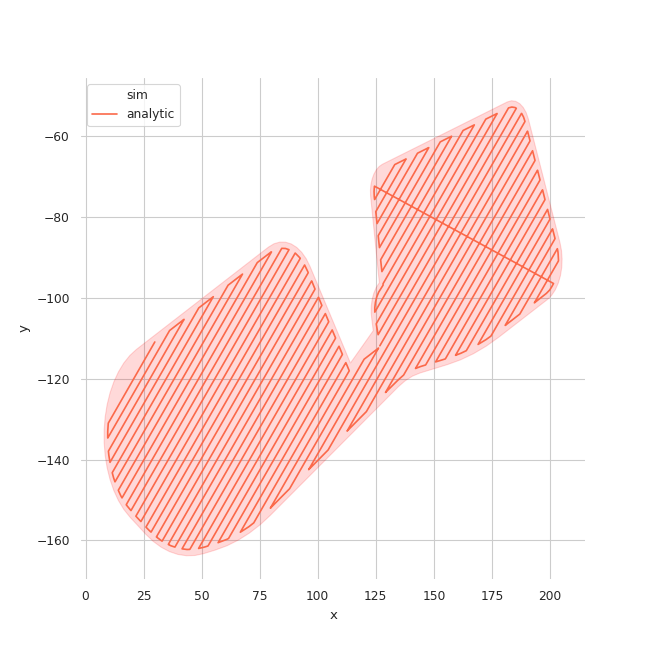
\includegraphics[width=\textwidth,trim=10 10 10 10,clip]{analytic_path.png}
\end{RoyalFigure}

Figure~\ref{fig:cpp_analytic} is an ``analytical'' representation of the path generated by the Captain. Which is to
say, it is a path generated without simulated sensor noise. It will server as a baseline and shows if the applied
strategy is feasable. The starting point of the crawler is approximately at \( [26, -100]^T \). The Captain senses
the curved corner on his right and nothing on its left. He continues on his arbitrary direction untill he senses a
wall in front of him. He continues to approach that wall to an acceptable distance before turning to the left; The
side where he sensed no boundaries. Continuing on his path in the opposite direction.

This sequence will continue, until first crosses over into the other basin. He stores this position as a change in
environment and continues until he reaches the top most corner of the other basin. He will now turn left and generate
a path until he is in the top left corner of the second basin. From here he travels without dredging towards the
unexplored area, traversing the covered region, perpendicular to its path until it reaches a landmark point. From
which he will continue generation his coverage path, until he has covered the basin as a whole.

\begin{RoyalFigure}[htb, label=fig:coverage_wo_kalman]{CPP WITH/WITHOUT KALMAN FILTERING}
    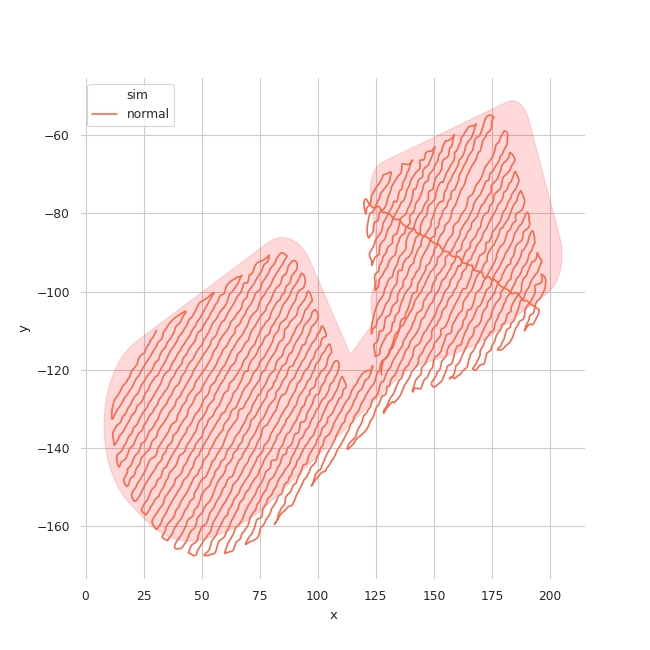
\includegraphics[width=0.5\textwidth,trim=10 10 10 10,clip]{normal_path.png}
    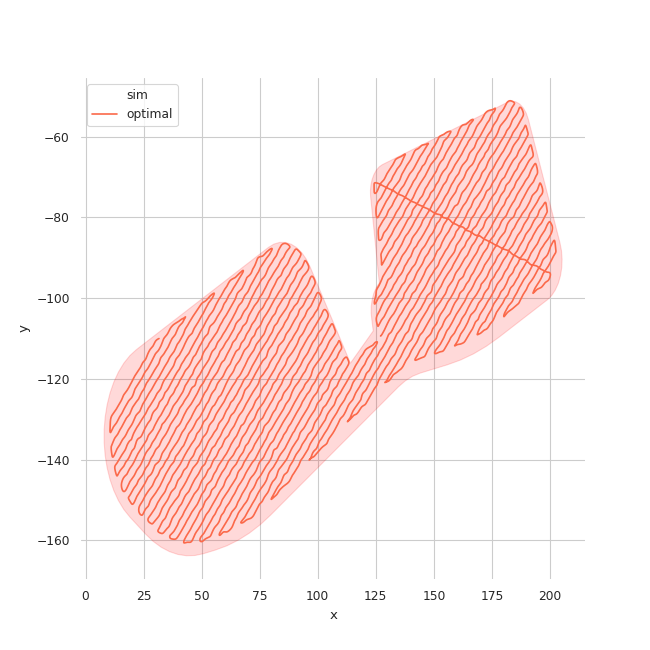
\includegraphics[width=0.5\textwidth,trim=10 10 10 10,clip]{optimal_path.png}
\end{RoyalFigure}

The \gls{acr-CPP} simulation is repeated two times, this time with sensor noise added. Simulating real life readings.
Showing both traveled paths in Figure~\ref{fig:coverage_wo_kalman}. These runs differ in concrete Navigator types. The
first run (shown on the left) is executed with a Navigator executing a simple \gls{acr-PID} algorithm. While the
second run uses an \gls{acr-UKF} (shown on the right). A first glance comparision gives a clear indication between the
differences.

The location error for a \gls{acr-PID} Navigator grows increasingly, letting the Captain think he's still within
the defined shore boundaries, while he is actually giving the beach goers the scare of their life. This happens due
to the simplification that was put into effect. Allowing boundaries to be ignored. Resulting in a longer duration in
which the development over time for the \gls{acr-NEES} can be compared. Which, is an important benchmark.

There are a few artifacts of note to point out in the \gls{acr-PID} controlled simulation. These occur due it's
low performance of filtering noise and compensating for certain sensor characteristics, such as: drift, bias and
transformations. The effects of noise become evident it the jagged lines. Which are, for illustration purposes
filter by decimation. The drift in signal obtained from the \gls{gls-gyroscope}, is showing in the divergence
of the back-and-forth paths. The effects are most clear in the upper right corner. An other artifact of sensor
characteristic behavior, which translates in a traveled path, is a difference in absolute path length. This is
systematically under estimated.

\begin{RoyalFigure}[htb, label=fig:NEES_kalman]{NEES OF THE CONTROLLER}
    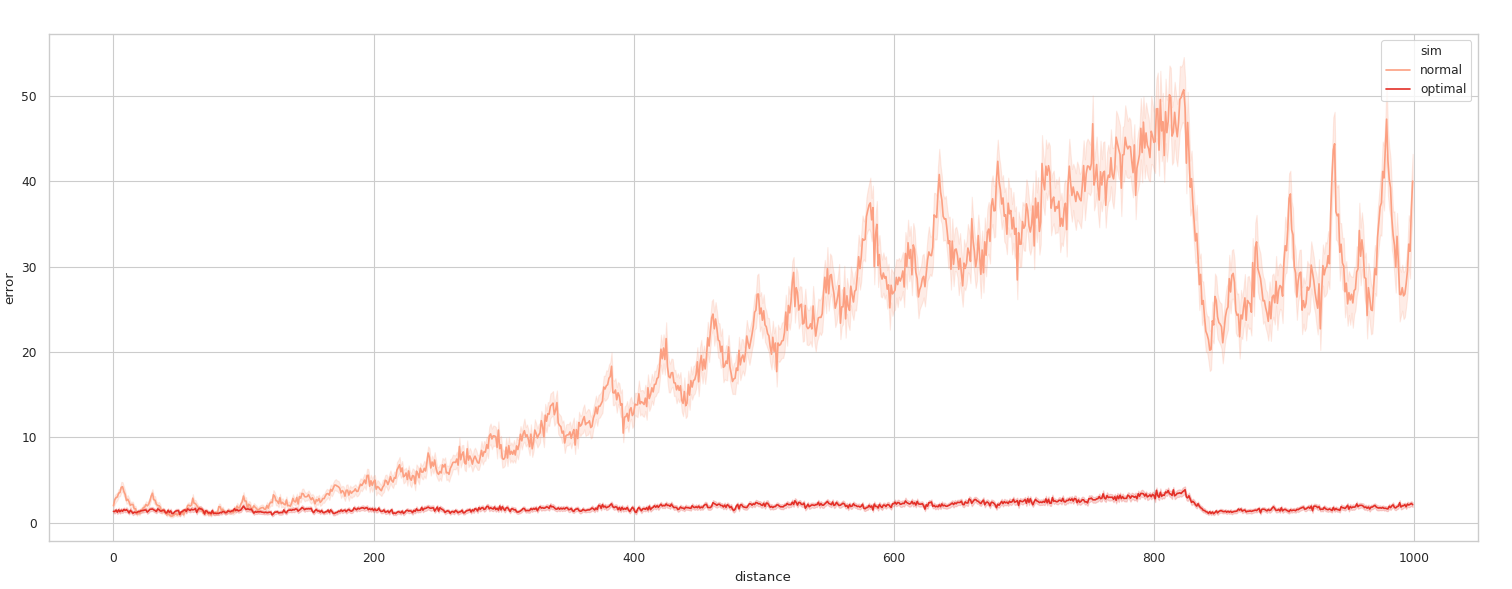
\includegraphics[width=\textwidth,trim=10 10 10 10,clip]{NEES_compared.png}
\end{RoyalFigure}

The above described artifacts are, to a lesser extend, also present in the second run. Which implements a
Navigator running a \gls{acr-UKF} algorithm. With an added benefit that this crawler doesn't turn into beach going
pshycokiller. Terrorizing unsuspecting families on a beach, by reenacting the scene from Godzilla emerging from the
ocean. There is still a growing error compared to the ``analytical'' position, but Figure~\ref{fig:NEES_kalman}
shows a clear difference between the performance of both controllers. The dip in signal around \( 800 \) is because
it encouters a distinct landmark feauture, which acts as a ground truth. A reference point used by the Captain from
which to track the traveled progress anew.